\documentclass{beamer}
\usepackage{pgfplots}
\pgfplotsset{compat=1.18}
\begin{document}
\begin{frame}{Columns}
\begin{columns}
\begin{column}{0.45\textwidth}
Some text next to the plot. It explains the data.
\end{column}
\begin{column}{0.5\textwidth}
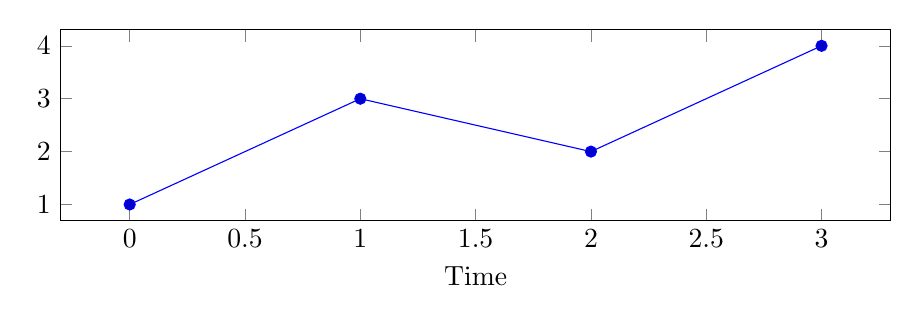
\begin{tikzpicture}
\begin{axis}[width=\columnwidth, height=4cm, xlabel={Time}]
\addplot coordinates {(0,1) (1,3) (2,2) (3,4)};
\end{axis}
\end{tikzpicture}
\end{column}
\end{columns}
\end{frame}
\end{document}
